\documentclass[12pt,letterpaper]{article}
\usepackage[utf8]{inputenc}
\usepackage[spanish]{babel}
\usepackage{graphicx}
\usepackage[left=2cm,right=2cm,top=2cm,bottom=2cm]{geometry}
\usepackage{graphicx} % figuras
% \usepackage{subfigure} % subfiguras
\usepackage{float} % para usar [H]
\usepackage{amsmath}
%\usepackage{txfonts}
\usepackage{stackrel} 
\usepackage{multirow}
\usepackage{enumerate} % enumerados
\renewcommand{\labelitemi}{$-$}
\renewcommand{\labelitemii}{$\cdot$}
% \author{}
% \title{Caratula}
\begin{document}

% Fancy Header and Footer
% \usepackage{fancyhdr}
% \pagestyle{fancy}
% \cfoot{}
% \rfoot{\thepage}
%

% \usepackage[hidelinks]{hyperref} % CREA HYPERVINCULOS EN INDICE
  
% \author{}
\title{Caratula}

\begin{titlepage}
    \begin{center}
    \begin{figure}[htb]
    \begin{center}
    
\includegraphics[width=3.5cm]{./img/upt.jpg}
    \end{center}
    \end{figure}
    
    \vspace*{0.15in}
    \begin{Large}
    \textbf{UNIVERSIDAD PRIVADA DE TACNA}\\
    \end{Large}
    
    \vspace*{0.1in}
    \begin{Large}
    \textbf{FACULTAD DE INGENIERIA} \\
    \end{Large}
    
    \vspace*{0.1in}
    \begin{Large}
    \textbf{ESCUELA PROFESIONAL DE INGENIERIA DE SISTEMAS} \\
    \end{Large}
    
    \vspace*{0.5in}
    \begin{Large}
    \textbf{TITULO:}\\
    \end{Large}
    

\vspace*{0.1in}
\begin{Large}
    Visualización de datos con TableauArchivo \\
\end{Large}

\vspace*{0.3in}
\begin{Large}
\textbf{Curso:} \\
\end{Large}

\vspace*{0.1in}
\begin{large}
    Inteligencia De Negocios\\
\end{large}

\vspace*{0.3in}
\begin{Large}
\textbf{Docente:} \\
\end{Large}

\vspace*{0.1in}
\begin{large}
Ing. Patrick Cuadros Quiroga\\
\end{large}

\vspace*{0.2in}
\vspace*{0.1in}
\begin{large}
\textbf{Alumno:} \\
\begin{flushleft}
    Cancino Tapia, Luis Antonio		\hfill	(2015052383) \\


\end{flushleft}
\end{large}
\vspace*{0.1in}
\begin{large}
Tacna - Perú\\
\end{large}
\vspace*{0.1in}
\begin{large}
2021\\
\end{large}

\end{center}

\end{titlepage}




\thispagestyle{empty} % INDICE SIN NUMERO
\newpage
\setcounter{page}{1} % REINICIAR CONTADOR DE PAGINAS DESPUES DEL INDICE



\section*{Laboratorio 03: Creando un Reporte Interactivo en Power BI}
\subsection*{Objetivo} 
Construir modelos de datos y reportes interactivos con Power BI conectándote a las principales fuentes de datos de tu organización. 
\\\\Evaluar un proyecto de Business Intelligence con Power BI teniendo en cuenta buenas prácticas y las características de esta completa suite de analítica de negocios.

\subsection*{Requerimientos}
Conocimientos \\\\
Para el desarrollo de esta práctica se requerirá de los siguientes conocimientos básicos: 
\\\\
- Conocimientos básicos de administración de base de datos Microsoft SQL Server. 
\\\\
- Conocimientos básicos de SQL.
\\\\
Software \\\\
Asimismo, se necesita los siguientes aplicativos: 
\\\\
- Microsoft SQL Server 2016 o superior 
\\\\
- Base de datos AdventureWorksLT2016 o superior
\\\\
- Tener los archivos de recursos del laboratorio. 
\\\\
- Power BI Desktop. 
\\\\
- Tener una cuenta Microsoft registrada en el Portal de Power Bi. 
\\\\



\subsection*{Desarollo}
Iniciar Power BI Desktop.
\begin{center}
    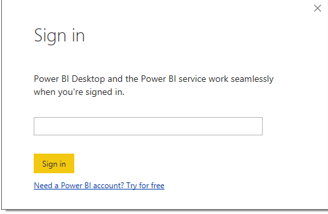
\includegraphics[width=16cm]{img/1.png}  
\end{center}
Cuando la Ventana de Power BI Desktop aparezca, en el panel a mano izquierda, hacer click en Obtener
Datos (Get Data).
\begin{center}
    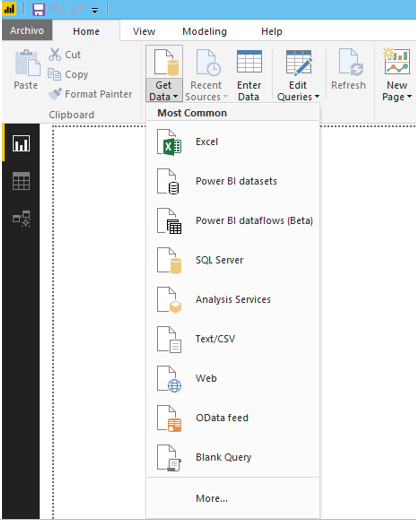
\includegraphics[width=16cm]{img/2.png}  
\end{center}
En el cuadro de dialogo Obtener Datos (Get Data), click en base de datos SQL Server, y luego hacer click en
Conectar (Connect).
\begin{center}
    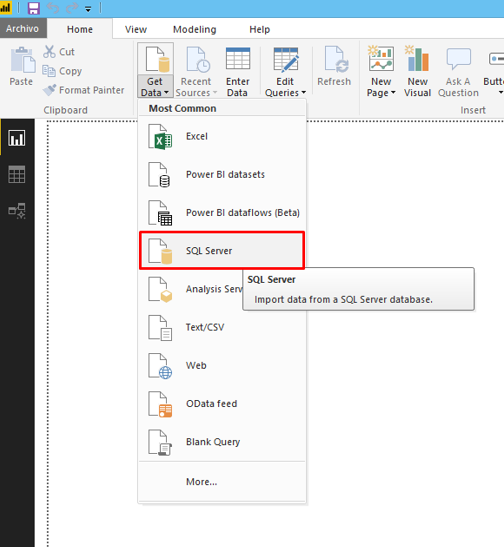
\includegraphics[width=16cm]{img/3.png}  
\end{center}
En el cuadro de dialogo base de datos SQL Server, en la casilla servidor tipear (local), en la casilla Base de
datos (opcional) / Database (optional), tipear AdventureWorks2017, y hacer clic en OK.

\begin{center}
    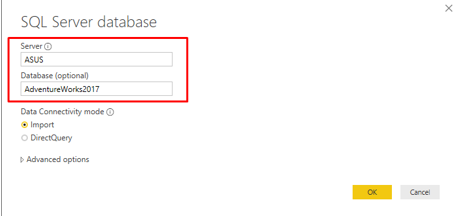
\includegraphics[width=16cm]{img/4.png}  
\end{center}
En el cuadro de dialogo base de datos SQL Server, aceptar los valores por defecto, y luego click en el
Conectar (Connect). Si un mensaje de Soporte de Encriptación es visualizado, hacer click en OK.
\begin{center}
    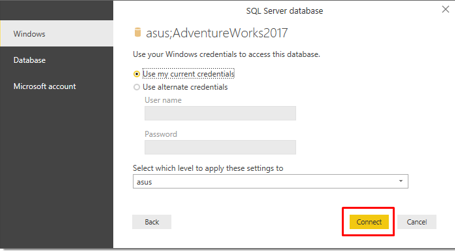
\includegraphics[width=16cm]{img/5.png}  
\end{center}
\begin{center}
    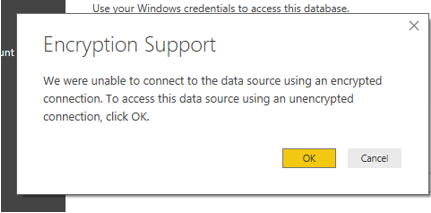
\includegraphics[width=16cm]{img/6.png}  
\end{center}
En el cuadro de dialogo Navegador (Navigator), seleccionar el check en Sales.vSalesPerson, y entonces hacer
click en Cargar (Load).
\begin{center}
    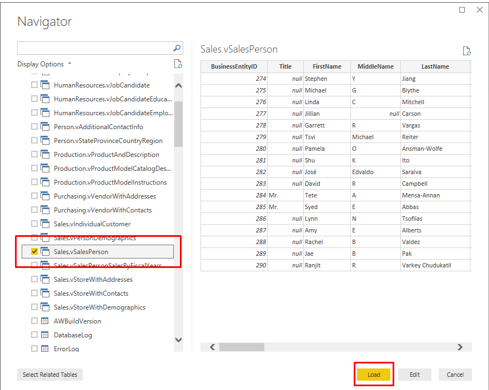
\includegraphics[width=16cm]{img/7.png}  
\end{center}
En el panel Campos (Fields), expandir Sales vSalesPerson para ver todas las columnas.
\begin{center}
    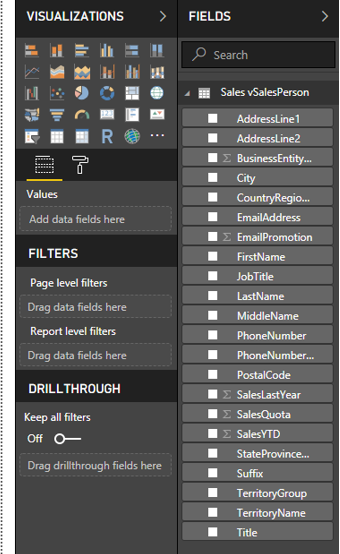
\includegraphics[width=16cm]{img/8.png}  
\end{center}
En el menu principal (Home ribbon), hacer click en Funetes Recientes (Recent Sources), y en local:
AdventureWorks2017.
\begin{center}
    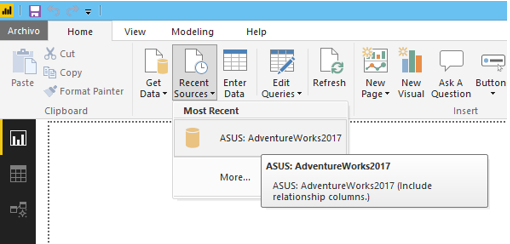
\includegraphics[width=16cm]{img/9.png}  
\end{center}
En el cuadro de dialogo Navegador (Navigator), seleccionar la vista Sales.vStoreWithDemographics, y luego
hacer click en Cargar (Load).
\begin{center}
    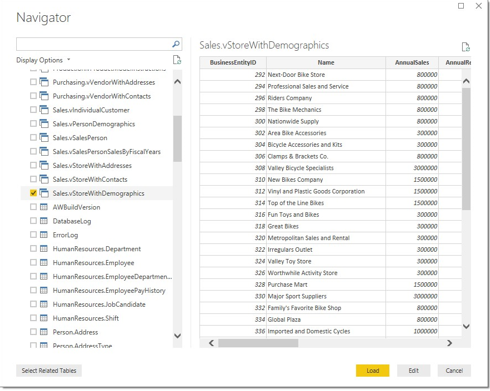
\includegraphics[width=16cm]{img/10.png}  
\end{center}
En el panel Campos (Fields), expandir Sales.vStoreWithDemographics para ver todas las columnas.
\begin{center}
    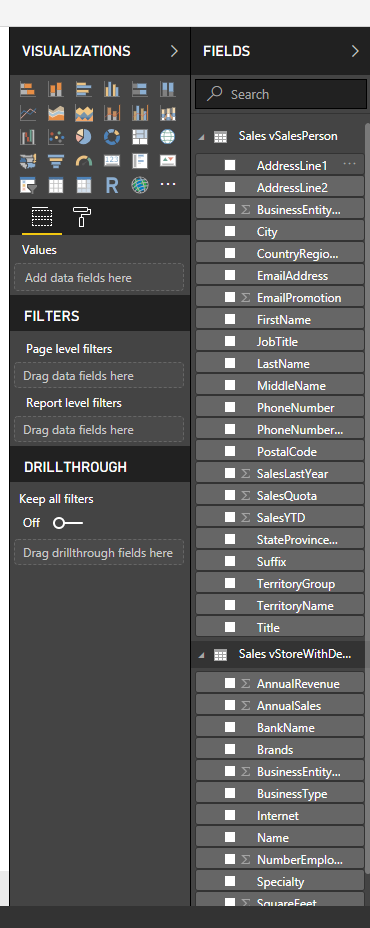
\includegraphics[width=10cm,height=22cm]{img/11.png}  
\end{center}
En el menu principal (Home ribbon), hacer click en Obtener Datos (Get Data), y luego click en SQL Server.
\begin{center}
    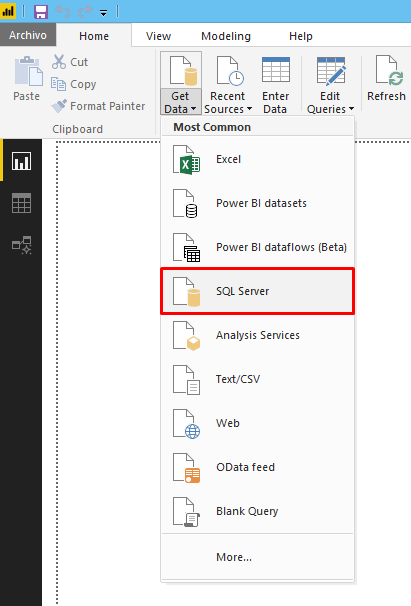
\includegraphics[width=16cm]{img/12.png}  
\end{center}
En el cuadro dialogo base de datos SQL Server, en la casilla Servidor (Server), tipear (local), y en la casilla
\begin{center}
    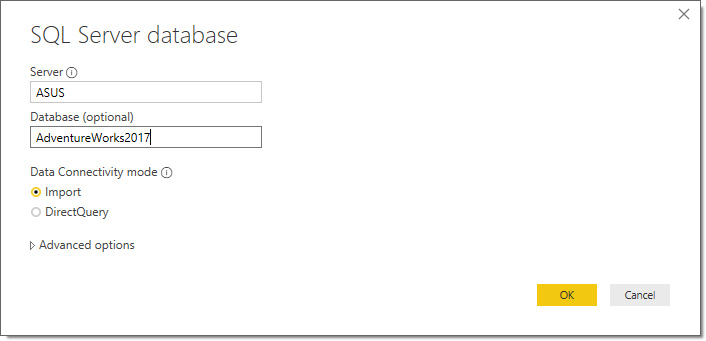
\includegraphics[width=10cm]{img/13.png}  
\end{center}
Base de datos (opcional), tipear AdventureWorks2016.\\\\
Expandir opciones Avanzadas, en la casilla sentencia SQL (opcional, base de datos requerida). 
\begin{center}
    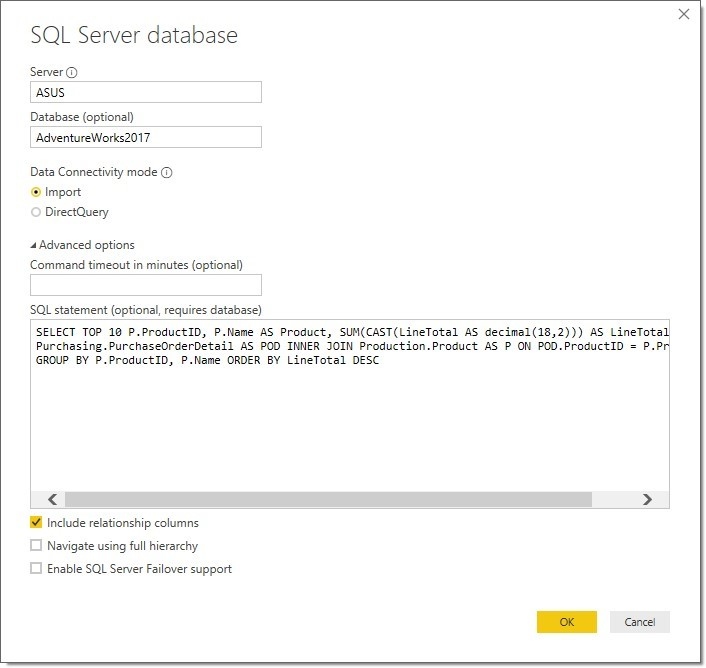
\includegraphics[width=10cm]{img/14.jpg}  
\end{center}
Si la Ventana Configuración de la Conexión (Connection Settings) aparece, hacer click en OK.
En el cuadro de dialogo (local): AdventureWorks2017 hacer click en Cargar (Load).
\begin{center}
    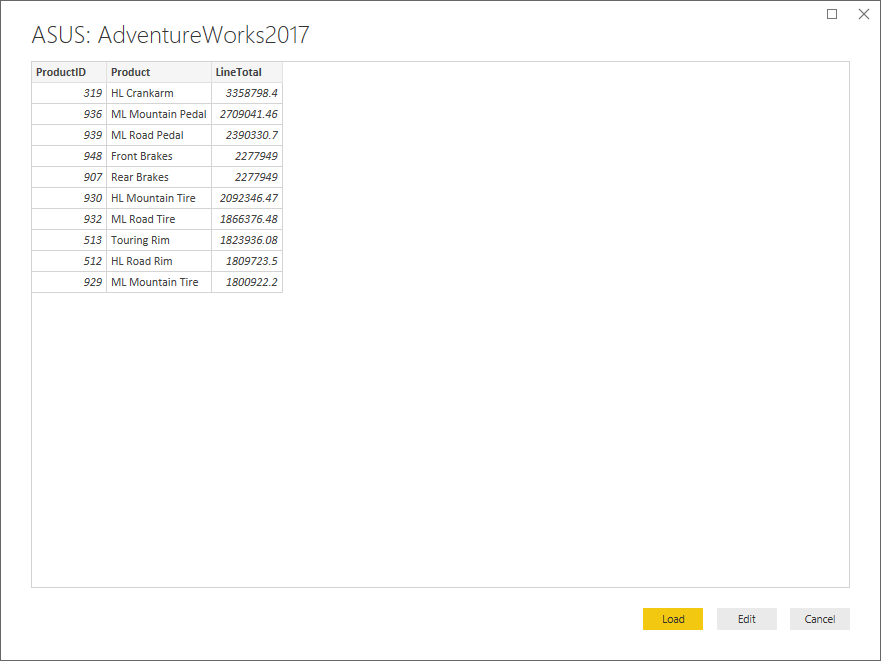
\includegraphics[width=16cm]{img/15.png}  
\end{center}
En el panel Campos, expander Query1 para ver todas las columnas.
\begin{center}
    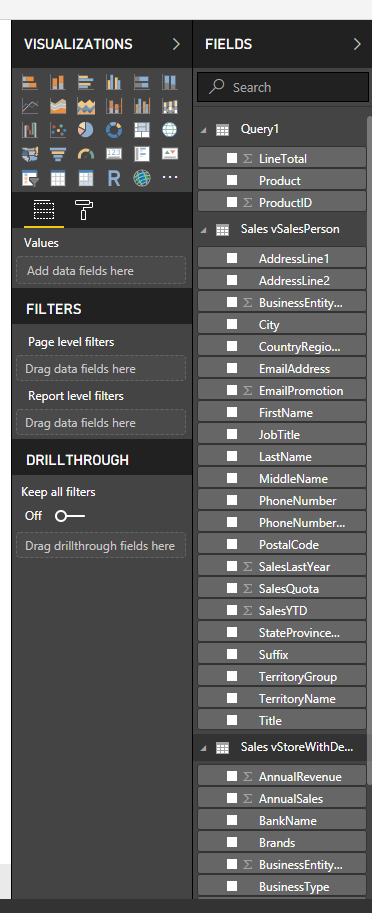
\includegraphics[width=10cm,height=22cm]{img/16.png}  
\end{center}
Hacer click en la elipsis (…) al lado de Query1 y hacer click en Renombrar, tipear Top 10 Productos
\begin{center}
    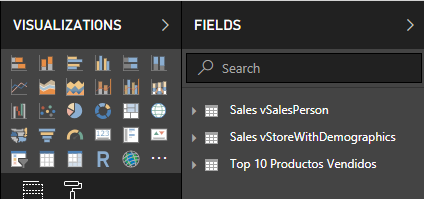
\includegraphics[width=16cm]{img/17.png}  
\end{center}
Adicionar Gráficos al Reporte\\\\
En el panel Visualizaciones (Visualizations), hacer click en el gráfico Columna apilada (Stacked column) para añadir el control al reporte.
\begin{center}
    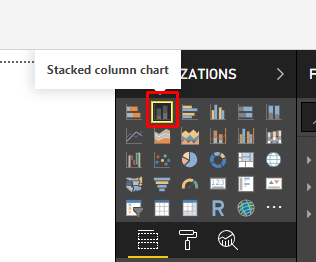
\includegraphics[width=16cm]{img/18.png}  
\end{center}
En el panel Campos (Fields), bajo Sales vSalesPerson, arrastrar el campo FirstName a la casilla Eje (Axis) en el panel de Visualización (Visualizations).
\begin{center}
    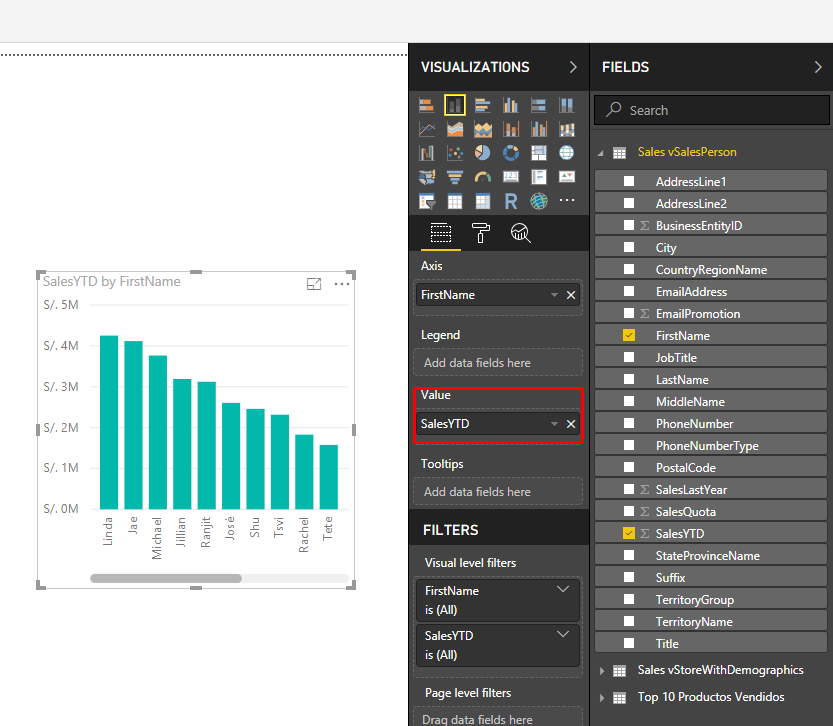
\includegraphics[width=16cm]{img/20.png}  
\end{center}
Arrastrar el campo SalesYTD a la casilla Valores (Values). El gráfico se llenará con datos.
\begin{center}
    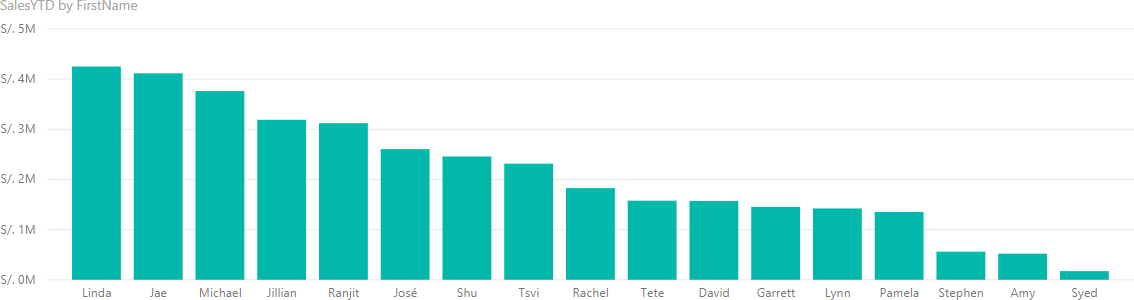
\includegraphics[width=16cm]{img/21.png}  
\end{center}
Asegurarse que el gráfico tiene el foco y luego ir al panel de Visualización (Visualizations), hacer click en la pestaña Formato (Format).
\begin{center}
    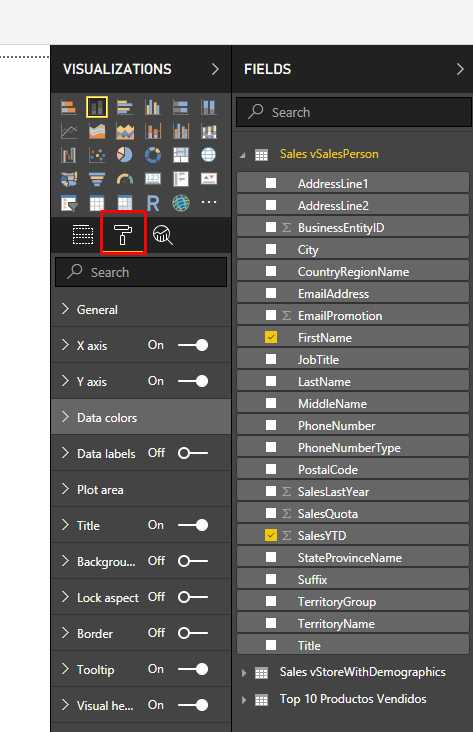
\includegraphics[width=16cm]{img/22.png}  
\end{center}
Expandir Colores de datos (Data colors), activar la opción Mostrar todos (Show all).
\begin{center}
    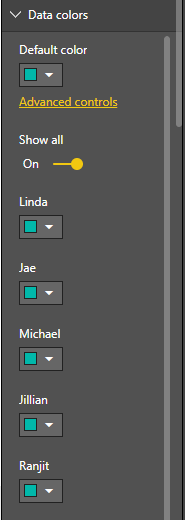
\includegraphics[width=10cm,height=25cm]{img/23.png}  
\end{center}
\begin{center}
    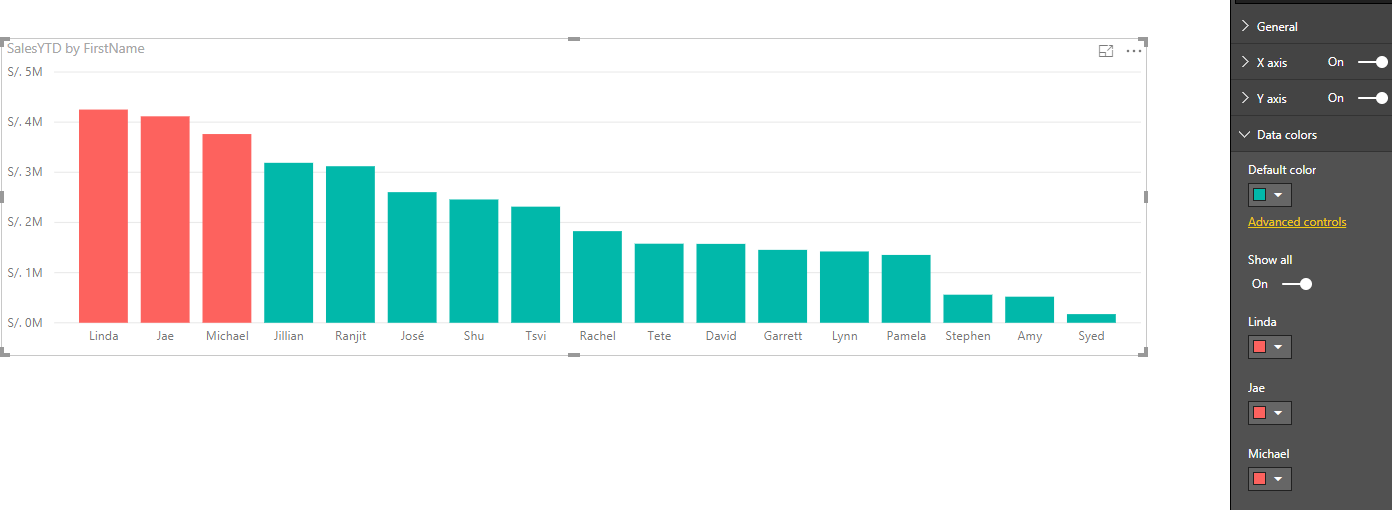
\includegraphics[width=16cm]{img/24.png}  
\end{center}
\end{document}

